\documentclass[thesis.tex]{subfiles}

\begin{document}
    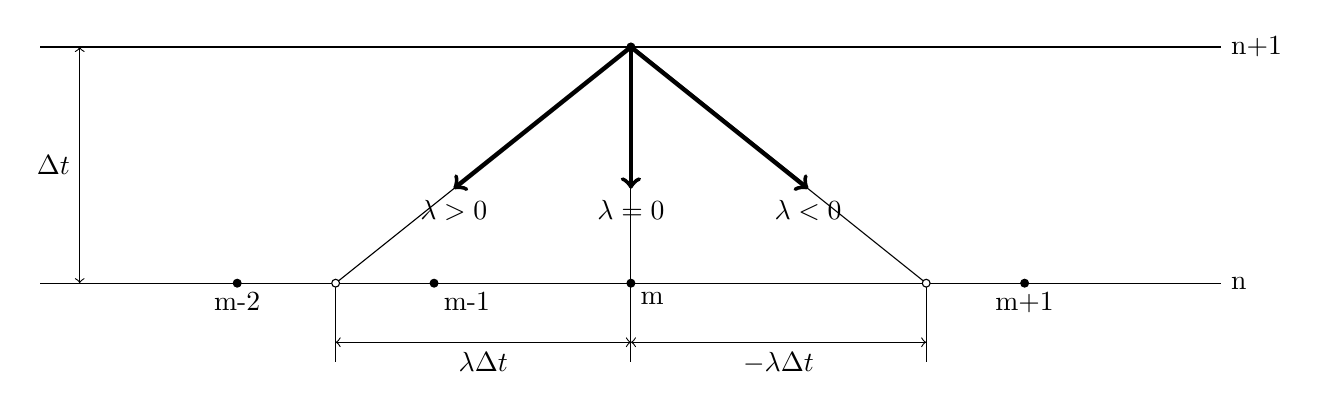
\begin{tikzpicture}
        % старый временной слой
        \draw (-7.5,0) -- (7.5,0) node[at end,right] {n};

        % новый временной слой
        \draw (-7.5,3) -- (7.5,3) node[at end,right] {n+1};

        % характеристики
        \draw (0,3) -- (-3.75, 0);
        \draw[ultra thick,->] (0,3) -- (-2.25,1.2)  node[at end, below] {$\lambda > 0$};
        \draw (0,3) -- (3.75, 0);
        \draw[ultra thick,->] (0,3) -- (2.25,1.2) node[at end, below] {$\lambda < 0$};
        \draw (0,3) -- (0, 0);
        \draw[ultra thick,->] (0,3) -- (0,1.2) node[at end, below] {$\lambda=0$};

        % шаг
        \draw (-3.75,0) -- (-3.75,-1);
        \draw (0,0) -- (0,-1);
        \draw[<->] (-3.75, -0.75) -- (0, -0.75) node[midway,below] {$\lambda\Delta t$};
        \draw (3.75,0) -- (3.75,-1);
        \draw[<->] (3.75, -0.75) -- (0, -0.75) node[midway,below] {$-\lambda\Delta t$};

        % точки
        \node[draw,circle,inner sep=1pt,fill] at (-5,0) {} node[below] at (-5,0) {m-2};
        \node[draw,circle,inner sep=1pt,fill] at (-2.5,0) {} node[below right] at (-2.5,0) {m-1};
        \node[draw,circle,inner sep=1pt,fill] at (0,0) {} node[below right] at (0,0) {m};
        \node[draw,circle,inner sep=1pt,fill] at (5,0) {} node[below] at (5,0) {m+1};
        \node[draw,circle,inner sep=1pt,fill] at (0,3) {};

        \node[draw,circle,inner sep=1pt,fill=white] at (-3.75,0) {};
        \node[draw,circle,inner sep=1pt,fill=white] at (3.75,0) {};

        \draw[<->] (-7,0) -- (-7,3) node[midway, left] {$\Delta t$};
    \end{tikzpicture}
\end{document}
